\documentclass{article}
\usepackage[a4paper, hmargin={2.5cm, 2.5cm}, vmargin={2.5cm, 2.5cm}]{geometry}
\usepackage[utf8]{inputenc}
\usepackage[english]{babel}
\usepackage{amsmath,amssymb,graphicx}
\usepackage{cleveref}
\usepackage{hyperref}

\usepackage{mathtools}
\usepackage{fancyhdr}
\usepackage{lastpage}
\usepackage{geometry}
\usepackage{ulem}
\usepackage{gauss}
\usepackage{graphicx}
\usepackage{pdfpages}
\usepackage{hyperref}
\usepackage{cleveref}
\usepackage{wrapfig}
\usepackage{morefloats}
\usepackage{upquote}


%%%%%% COLORS %%%%%%%%

\usepackage{xcolor}
\definecolor{red1}{rgb}{0.7, 0.0, 0.3}
\definecolor{red2}{rgb}{0.5, 0.0, 0.5}
\definecolor{red3}{rgb}{0.3, 0.0, 0.7}

%two definitions of the color grey
\usepackage{color}
\definecolor{listinggray}{gray}{0.9}
%\definecolor{lbcolor}{rgb}{0.9,0.9,0.9}

\usepackage{listings}
\lstset{
	language=Python,
	literate=
		{æ}{{\ae}}1
		{ø}{{\o}}1
		{å}{{\aa}}1
		{Æ}{{\AE}}1
		{Ø}{{\O}}1
		{Å}{{\AA}}1
		{'}{{'}}1,
	backgroundcolor=\color{listinggray},
	tabsize=3,
	rulecolor=,
	basicstyle=\scriptsize,
	upquote=true,
	aboveskip={1.5\baselineskip},
	columns=fixed,
	showstringspaces=false,
	extendedchars=true,
	breaklines=true,
	prebreak =\raisebox{0ex}[0ex][0ex]{\ensuremath{\hookleftarrow}},
	frame=single,
	showtabs=false,
	showspaces=false,
	showstringspaces=false,
	identifierstyle=\ttfamily,
	keywordstyle=\color[rgb]{0,0,1},
	commentstyle=\color[rgb]{0.133,0.545,0.133},
	stringstyle=\color[rgb]{0.627,0.126,0.941},
}

\lstset{moredelim=[s][\color{gray}]{(*}{*)}}
\lstset{morecomment=[l][\color{gray}]{##}}
\lstset{moredelim=[s][\color{green!50!brown}]{"}{"}}
\lstset{moredelim=[s][\color{green!50!brown}]{'}{'}}
\lstset{moredelim=[s][\color{gray}]{/*}{*/}}

\lstset{literate=
	{0}{{{\color{violet}{0}}}}1
	{1}{{{\color{violet}{1}}}}1
	{2}{{{\color{violet}{2}}}}1
	{3}{{{\color{violet}{3}}}}1
	{4}{{{\color{violet}{4}}}}1
	{5}{{{\color{violet}{5}}}}1
	{6}{{{\color{violet}{6}}}}1
	{7}{{{\color{violet}{7}}}}1
	{8}{{{\color{violet}{8}}}}1
	{9}{{{\color{violet}{9}}}}1
	{?}{{{\color{orange}{?}}}}1
}

\lstset{emph={for, in, if, elif, else, return, def, print}, emphstyle={\color{blue}},,,
        emph={[3]std}, emphstyle={[3]\color{green}}}

\lstset{emph={True, False}, emphstyle={\color{violet}},,
        emph={[3]std}, emphstyle={[3]\color{green}}}

%captions on listings
\usepackage[center,font=small,labelfont=bf,textfont=it]{caption}

\title{Insert Assignment Title Here\\02807 Computational Tools for Big Data}
\author{Anonymous authors}
\date{
	\today
}

\setlength\parindent{0pt}		% noindent through whole document
\usepackage[parfill]{parskip}	% extra linebreak on new paragraph

\begin{document}

\maketitle

\section{Week 8: Map Reduce}

\subsection{Exercise 1}
\label{sub:Exercise 1}

We chose the following small text string to illustrate counting words:

\begin{lstlisting}
this test tests a test
\end{lstlisting}

We used the following code to find word count:

\begin{lstlisting}[language=Python]
class exercise_1(MRJob):
    def mapper(self, _, line):
        for word in line.split():
            yield word, 1

    def reducer(self, key, values):
        yield key, sum(values)
\end{lstlisting}

Which yielded the following output:

\begin{lstlisting}
"a"	1
"test"	2
"tests"	1
"this"	1
\end{lstlisting}

We notice that "test" was correctly counted as occuring twice.

\subsection{Exercise 2}
\label{sub:Exercise 2}

We ran the following code against all of the given test graphs.

\begin{lstlisting}
class exercise_2(MRJob):
    def steps(self):
        return [
            MRStep(
                mapper=self.mapper,
                reducer=self.reducer
            ),
            MRStep(
                reducer=self.combine_reduced_values
            )
        ]

    def mapper(self, _, line):
        for word in line.split():
            yield word, 1

    def reducer(self, key, values):
        yield None, sum(values) % 2 == 0

    def combine_reduced_values(self, _, values):
        yield "Does an Euler tour exist?", self.is_list_true(values)

    def is_list_true(self, l):
        is_true = True
        for x in l:
            is_true = is_true and x
        return is_true
\end{lstlisting}

And get the following output:

\begin{lstlisting}
"Does an Euler tour exist?"	true (euler_graph_1.txt)
"Does an Euler tour exist?"	false (euler_graph_2.txt)
"Does an Euler tour exist?"	true (euler_graph_3.txt)
"Does an Euler tour exist?"	true (euler_graph_4.txt)
"Does an Euler tour exist?"	false (euler_graph_5.txt)
\end{lstlisting}

\subsection{Exercise 3}
\label{sub:Exercise 3}

We solve the problem of finding the list of friends of friends using the following code:

\begin{lstlisting}
class exercise_3(MRJob):
    def steps(self):
        return [
            MRStep(
                mapper=self.mapper,
                reducer=self.friend_pairs
            ),
            MRStep(
                reducer=self.friend_intersection
            )
        ]

    def mapper(self, _, line):
        user, friend = line.split()
        yield int(user), int(friend)
        yield int(friend), int(user)  # make sure we have the opposite relation from B to A

    def friend_pairs(self, user, friends):
        friend_list = reduce(lambda x, y: x + [y], friends, [])

        for friend in friend_list:
            yield sorted([user, friend]), friend_list

    def friend_intersection(self, friend_pair, combined_friends):

        combined_friends = reduce(lambda x, y: x + [y], combined_friends, [])
        intersection = []

        for friend in combined_friends[0]:
            if friend in combined_friends[1]:
                intersection += [friend]

        yield friend_pair, intersection
\end{lstlisting}

This code outputs data listing all friends of friends in the following format:

\begin{lstlisting}
	...
[0, 100]	[119, 150, 163, 189, 217, 269, 323, 64]
[0, 101]	[180, 187, 194, 204, 24, 242, 249, 254, 266, 299, 302, 317, 330, 346, 53, 80, 92, 94]
[0, 102]	[175, 227, 263, 296, 99]
[0, 103]	[136, 169, 172, 185, 200, 211, 25, 252, 271, 285, 323, 339, 56, 7, 98]
[0, 104]	[109, 113, 122, 123, 128, 142, 169, 186, 188, 200, 203, 21, 212, 239, 25, 252, 26, 271, 277, 295, 303, 318, 322, 325, 332, 344, 45, 55, 56, 67, 98]
[0, 105]	[119, 148, 21, 236, 25, 257, 272, 277, 280, 315, 39, 69, 9]
[0, 106]	[169, 231, 238, 29, 329, 332, 88]
[0, 107]	[171, 58]
[0, 108]	[127, 159, 184, 197, 21, 251, 272, 281, 284, 320, 36, 57]
[0, 109]	[104, 118, 119, 122, 13, 142, 148, 158, 169, 186, 200, 203, 21, 229, 239, 252, 26, 271, 277, 285, 295, 297, 303, 304, 31, 314, 322, 323, 324, 325, 331, 332, 50, 56, 67, 98]
	...
\end{lstlisting}

Where the first list is the sorted list of user id's, and the second list is the list of friends these two users have in common. We did not supply the complete output since it is quite large.

\subsection{Exercise 4}
\label{sub:Exercise 4}

For finding the number of triangles in a graph we used the following code:

\begin{lstlisting}
class exercise_4(MRJob):
    def steps(self):
        return [
            MRStep(
                mapper=self.mapper,
                reducer=self.reducer
            ),
            MRStep(reducer=self.discover_triangles),
            MRStep(reducer=self.count_triangles),
            MRStep(reducer=self.sum_triangles)
        ]

    def mapper(self, _, line):
        node_a, node_b = line.split()
        yield int(node_a), int(node_b)
        yield int(node_b), int(node_a)

    def reducer(self, node, connecting_nodes):
        """
        We return a tuple of two connecting nodes and their respective connecting nodes in a list:
             (node_a, node_b), [(node_a, nodes), (node_b, nodes)]
        :param node:
        :param connecting_nodes:
        """
        nodes = reduce(lambda x, y: x + [y], connecting_nodes, [])

        for n in nodes:
            yield sorted([node, n]), (n, nodes)

    def discover_triangles(self, node_pair, connecting_nodes):
        """
        We have all nodes associated with both nodes in node_pair (connecting_nodes)
        If both nodes in node_pair have the same connecting node, they must form a triangle
        :param node_pair:
        :param connecting_nodes:
        """
        node_a, node_b = node_pair
        common_nodes = []

        for node, nodes in connecting_nodes:
            for connected_node in nodes:
                if connected_node != node:
                    if connected_node in common_nodes:
                        # this yields True for every point in the triangle.
                        yield sorted([node_a, node_b, connected_node]), True
                    else:
                        common_nodes += [connected_node]

    def count_triangles(self, _, triangles):
        yield "triangles", 1

    def sum_triangles(self, _, triangles):
        yield _, sum(triangles)
\end{lstlisting}

Running this on the $roadNet-CA.mtx$ file (with headers removed) gives us the following output:

\begin{lstlisting}
"triangles"	120676
\end{lstlisting}

\section{Week 9: Apache Spark}

\subsection{Exercise 1}
\label{sub:Exercise 1}

We uploaded the following code to our apache spark IPython notebook:

\begin{lstlisting}
words = sc.textFile("data/cs100/lab1/words.txt")

counts = words.flatMap(lambda line: line.split(" ")) \
             .map(lambda word: (word, 1)) \
             .reduceByKey(lambda x, y: x + y)

counts.saveAsTextFile("data/cs100/lab1/words_count")
\end{lstlisting}

We run the code against the following file:

\begin{lstlisting}
this test tests a test
\end{lstlisting}

And we get the following result.

\begin{lstlisting}
(u'', 4)
(u'this', 1)
(u'tests', 1)
(u'test', 2)
(u'a', 1)
\end{lstlisting}

We notice here that the code was able to correctly count the number of occurrences of the word "test" in the given file.

\subsection{Exercise 2}
\label{sub:Exercise 2}

We uploaded the following code to our IPython spark notebook:

\begin{lstlisting}
graph1 = sc.textFile("data/exercise2/euler_graph_1.txt")
graph2 = sc.textFile("data/exercise2/euler_graph_2.txt")
graph3 = sc.textFile("data/exercise2/euler_graph_3.txt")
graph4 = sc.textFile("data/exercise2/euler_graph_4.txt")
graph5 = sc.textFile("data/exercise2/euler_graph_5.txt")

def euler_tour(words):
    return words.flatMap(
        lambda line: line.split(" ")
    ).map(
        lambda word: (word, 1)
    ).reduceByKey(
        lambda x, y: x + y
    ).map(
        lambda (x, y): y % 2 == 0
    ).reduce(
        lambda x, y: x and y
    )

print(euler_tour(graph1))
print(euler_tour(graph2))
print(euler_tour(graph3))
print(euler_tour(graph4))
print(euler_tour(graph5))
\end{lstlisting}

Running this code on the supplied graphs we get the following result:

\begin{lstlisting}
True
False
True
True
False
\end{lstlisting}

We notice that this result is in fact the same we found using mapreduce.

\subsection{Exercise 3}
\label{sub:Exercise 3}

We uploaded the following IPython notebook to the sparkvm.

\begin{lstlisting}
import ast

data = sc.textFile("data/exercise3/wifi.data")
data_objects = data.map(lambda x: ast.literal_eval(x))

def find_bssid(objects):
    return objects.map(
        lambda x: (x['bssid'], 1)
    ).reduceByKey(
        lambda x, y: x + y
    )

def find_ssid(objects):
    return objects.map(
        lambda x: (x['ssid'], 1)
    ).reduceByKey(
        lambda x, y: x + y
    )

def longest_ssid(objects):
    return objects.map(
        lambda x: ((x['bssid'], x['ssid']), len(x['ssid']))
    ).reduceByKey(
        lambda x, y: y
    )

print(find_bssid(data_objects).takeOrdered(10, key=lambda x: -x[1]))
print(find_ssid(data_objects).takeOrdered(10, key=lambda x: -x[1]))
print(longest_ssid(data_objects).takeOrdered(10, key=lambda x: -x[1]))
\end{lstlisting}

Running this code on the given dataset returned the following three result sets.

10 most common bssid's:

\begin{lstlisting}
[(u'34:21:09:12:6c:1a', 347),
 (u'00:24:b2:98:39:d2', 338),
 (u'34:21:09:12:6c:18', 324),
 (u'e8:08:8b:c9:c1:79', 318),
 (u'44:94:fc:56:08:fb', 315),
 (u'00:22:b0:b3:f2:ea', 314),
 (u'2c:b0:5d:ef:08:2b', 272),
 (u'44:94:fc:56:ce:5e', 240),
 (u'28:cf:e9:84:a1:c3', 211),
 (u'bc:ee:7b:55:1a:43', 210)]
\end{lstlisting}

10 most common ssid's:

\begin{lstlisting}
[(u'Kaspers Wi-Fi-netv\xe6rk', 402),
 (u'Internet4realz', 402),
 (u'AirLink5GHz126C18', 347),
 (u'NETGEAR_1', 338),
 (u'AirLink126C18', 324),
 (u'Housing People', 318),
 (u'Lausten_5GHz', 315),
 (u'Bronx', 314),
 (u'Playhouse', 272),
 (u'Lausten', 240)]
\end{lstlisting}

10 longest ssid's:

\begin{lstlisting}
[((u'f0:92:1c:a3:30:43', u'HP-Print-43-Deskjet 3520 series'), 31),
 ((u'08:76:ff:84:ff:8c', u'TeliaGateway08-76-FF-84-FF-8C'), 29),
 ((u'08:76:ff:8a:ee:32', u'TeliaGateway08-76-FF-8A-EE-32'), 29),
 ((u'08:76:ff:9c:e0:82', u'TeliaGateway08-76-FF-9C-E0-82'), 29),
 ((u'08:76:ff:46:3e:36', u'TeliaGateway08-76-FF-46-3E-36'), 29),
 ((u'9c:97:26:57:15:f9', u'TeliaGateway9C-97-26-57-15-F9'), 29),
 ((u'9c:97:26:57:15:99', u'TeliaGateway9C-97-26-57-15-99'), 29),
 ((u'a4:b1:e9:2c:9e:ca', u'TeliaGatewayA4-B1-E9-2C-9E-CA'), 29),
 ((u'08:76:ff:85:04:2f', u'TeliaGateway08-76-FF-85-04-2F'), 29),
 ((u'20:c9:d0:a3:54:9f', u'Charlotte R.s Wi-Fi-netv\xe6rk'), 27)]
\end{lstlisting}

\section{Week 10: Deep Learning}

\subsection{Exercise 1}

Deep Learning is a kind of Machine Learning, that focuses on using multiple layers of non-linear processing units. Deep learning is special in the way that algorithms designed for Deep Learning is based on distributed representations. This means that we make the assumption, that all observed data have been generated by different factors on the multiple layers of different levels of abstractions. Deep Learning was originally introduced with the object of moving Machine Learning closer to Artificial Intelligence, and has been used in the research community to solve big data problems such as speech recognition, computer vision, and natural language processing.


\subsection{Exercise 2}

Convolutional neural networks (CNN) is a kind of neural network, that takes advantage of being able to reuse copies of neurons. This way, it is possible to have a very large neural network, while keeping the number of parameters low. This is smart because this means, that the CNN has much fewer neurons, that needs to learn during learning. Copies of the neuron is then used multiple times in the convolution layer. This works much like how a function in programming is used multiple times instead of writing the code of the function multiple times.

We can have a neuron $a$, that we use multiple times, so that it collectively covers all input data, where each neuron covers multiple data points. This group of (identical) neurons, we call $A$, and it makes up the convolution layer. It is possible to have multiple layers, and with each new layer, the network can find more abstract features.

Convolution layers are often interweaved, so that $a_1 \leftarrow \{1, 2\}$ and $a_2 \leftarrow \{2, 3\}$, which makes for higher precision. However, from a high level perspective, it might not be needed to have a high level of precision. For this, max-pooling layers offers better performance (with the loss of precision). The way max-pooling layers works is that the neurons don't interweave, so we have $m_1 \leftarrow \{1, 2\}$ and $m_2 \leftarrow \{3, 4\}$.


\subsection{Exercise 3}

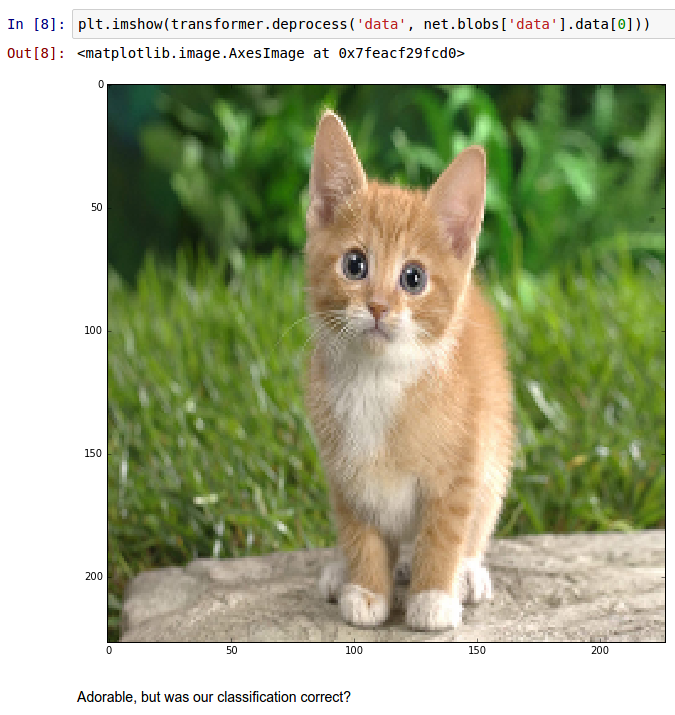
\includegraphics[scale=0.5]{cat.png}

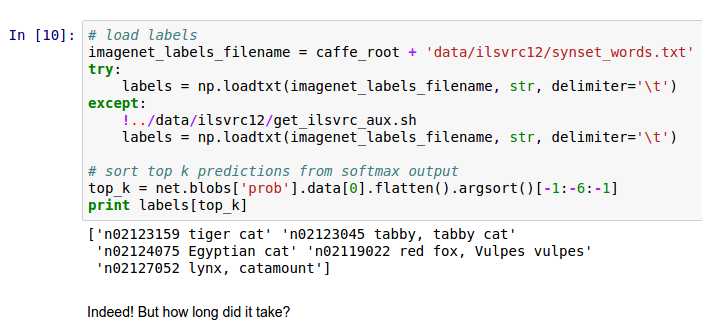
\includegraphics[scale=0.5]{cat2.png}

In the above classification of the cat from the assignment, you can see, that the classifier correctly guesses it is a cat (of some kind). All five guesses are cats (except for the fox, but I'll let it slide).

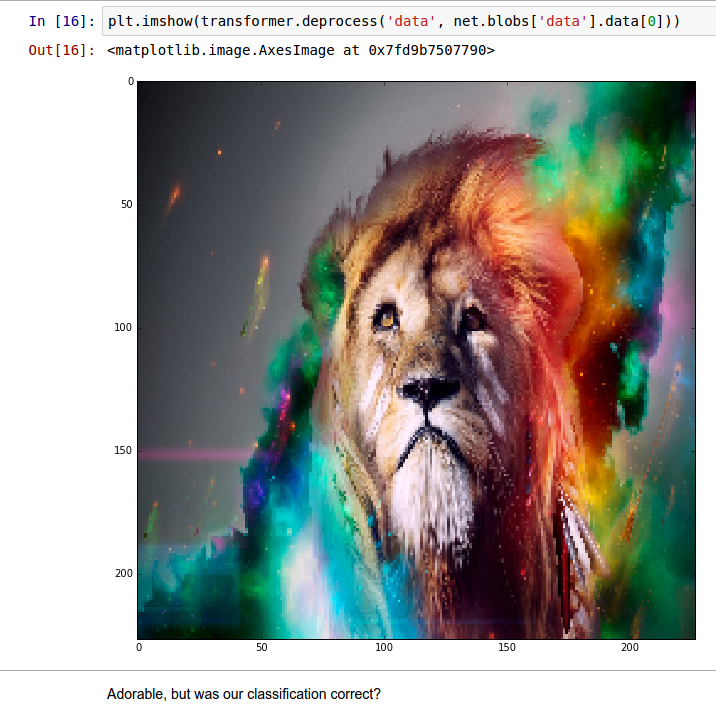
\includegraphics[scale=0.5]{lion1.png}

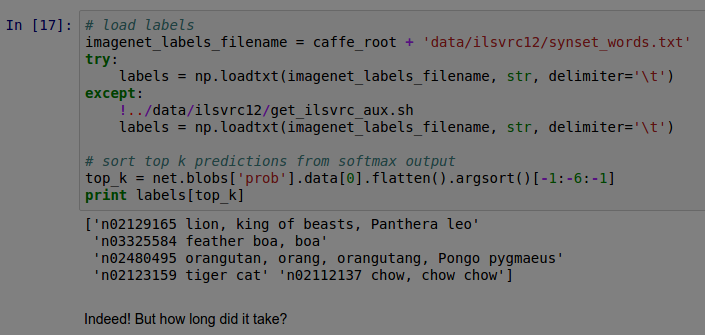
\includegraphics[scale=0.5]{lion2.png}

In the above classification, where we uploaded our own image, you can see, that the classifier correctly guesses a Lion. The next 3 guesses are off, and the fifth guess is somewhat okay. There will be a larger error margin, since the uploaded image is highly photoshopped and abstract.


\section{Week 11: Feature Hashing and LSH}

\subsection{Exercise 1}
\label{sub:Exercise 1}

\begin{lstlisting}
from __future__ import division
import hashlib
import json
from sklearn.ensemble import RandomForestClassifier as rfc


directory = "../../full/"


def bag_of_words(lines):

    uniq = set()

    for line in lines:
        # Iterate over all words
        for word in line[0].split():

            # Put words not already found into dictionary
            uniq.add(word)

    uniq_dict = {}
    for j, word in enumerate(uniq):
        uniq_dict[word] = j

    uniq_len = len(uniq)

    # Use word dictionary to create bag-of-words
    bag = []
    for line in lines:
        vec = [0] * uniq_len
        for word in line[0].split():
            vec[uniq_dict[word]] += 1
        bag.append((vec, (1 if 'earn' in line[1] else 0)))

    return bag


def bag_of_words_feature_hashed(lines, N):

    uniq = set()

    for line in lines:
        # Iterate over all words
        for word in line[0].split():

            # Put words not already found into dictionary
            uniq.add(word)

    uniq_dict = {}
    for j, word in enumerate(uniq):
        uniq_dict[word] = j

    # Use word dictionary to create bag-of-words
    bag = []
    for line in lines:
        vec = [0] * N
        for word in line[0].split():
            h = int(hashlib.md5(word).hexdigest(), 16) % N
            vec[h] += 1
        bag.append((vec, (1 if 'earn' in line[1] else 0)))

    return bag


if __name__ == "__main__":
    articles = []
    for i in range(21):
        f = open(directory + "reuters-0" + (str(i) if i >= 10 else "0" + str(i)) + ".json", 'r')
        articles += json.loads(f.read())
        f.close()

    articles = reduce(lambda x, y: x + ([y] if ('topics' in y.keys())
                                               and ('body' in y.keys())
                                               and (len(y['topics']) > 0)
                                               and (len(y['body']) > 0)
                                            else []), articles, [])

    lines = map(lambda x: (x['body'].lower().encode('ascii', errors='ignore'), x['topics']), articles)

    print "Calcualting bag of words."
    bow = bag_of_words(lines)
    print "Amount of lines: " + str(len(bow))
    print "Amount of words: " + str(len(bow[0][0]))

    training_set = bow[:int(round(len(bow)*0.8))]
    training_set_data = [row[0] for row in training_set]
    training_set_target = [row[1] for row in training_set]

    test_set = bow[-int(round(len(bow)*0.2)):]
    test_set_data = [row[0] for row in test_set]
    test_set_target = [row[1] for row in test_set]

    classifier = rfc(n_estimators=50)
    classifier.fit(training_set_data, training_set_target)
    predictions = classifier.predict(test_set_data)

    accuracy = []
    for i, prediction in enumerate(predictions):
        accuracy += [test_set_target[i] == prediction]
    accuracy = (accuracy.count(True) / len(test_set_target)) * 100

    print "Accuracy of classifier: " + str(accuracy) + "%"

    print "\nCalculating bag of words using feature hashing."
    bow = bag_of_words_feature_hashed(lines, 1000)
    print "Amount of lines: " + str(len(bow))
    print "Amount of words: " + str(len(bow[0][0]))

    training_set = bow[:int(round(len(bow)*0.8))]
    training_set_data = [row[0] for row in training_set]
    training_set_target = [row[1] for row in training_set]

    test_set = bow[-int(round(len(bow)*0.2)):]
    test_set_data = [row[0] for row in test_set]
    test_set_target = [row[1] for row in test_set]

    classifier = rfc(n_estimators=50)
    classifier.fit(training_set_data, training_set_target)
    predictions = classifier.predict(test_set_data)

    accuracy = []
    for i, prediction in enumerate(predictions):
        accuracy += [test_set_target[i] == prediction]
    accuracy = (accuracy.count(True) / len(test_set_target)) * 100

    print "Accuracy of classifier: " + str(accuracy) + "%"
\end{lstlisting}


\end{document}
